% 第6章第3节：基于正交矩阵的对角化（谱定理、Rayleigh商与谱的极值性质、对称矩阵的函数）。

\section{基于正交矩阵的对角化}
\label{sec:ls-spectral-theory}

上一节用可逆矩阵$\bm V$对角化，只要求基由特征向量组成，没有要求这些方向互相垂直。本节追问：哪些矩阵能用正交矩阵对角化，即找到一组标准正交的特征向量？答案是实对称矩阵，这一结论称为谱定理。有了这种分解，特征值还获得第二种含义：它们是二次型在单位球面上的极值，因此可以不求特征向量而比较、估计特征值。沿互相垂直的特征方向，还可以定义矩阵的平方根、对数等函数。

\subsection{谱定理}
\label{sec:ls-symmetric-spectral-decomposition}

先说明为什么希望特征方向互相垂直。若$\bm q_1,\ldots,\bm q_d$是$\mathbb R^d$的标准正交基，把它们排成正交矩阵$\bm Q$，则$\bm Q^{-1}=\bm Q^\top$。于是换基不必解方程：向量$\bm x$的新坐标就是内积$c_i=\bm q_i^\top\bm x$，长度也保持不变，$\lVert\bm x\rVert_2^2=\sum_ic_i^2$（第~\ref{sec:ls-orthonormal-bases}节）。所以，若方阵$\bm A$能写成$\bm A=\bm Q\bm\Lambda\bm Q^\top$，其中$\bm\Lambda$为实对角矩阵，它的作用就最容易看清：先用内积读出各方向的坐标，再把第$i$个坐标乘以$\lambda_i$，最后合回去。

哪些矩阵能这样写？必要条件很容易看出：若$\bm A=\bm Q\bm\Lambda\bm Q^\top$，则$\bm A^\top=\bm Q\bm\Lambda^\top\bm Q^\top=\bm A$，所以$\bm A$必须对称。对称矩阵也就是第~\ref{sec:ls-adjoints}节的自伴算子在标准坐标下的矩阵。本小节证明这一条件也是充分的。

下面把对称矩阵记为$\bm S$。证明的思路是：在单位球面上最大化二次型$\bm x^\top\bm S\bm x$，说明取到最大值的方向是一个特征方向，再在与它垂直的子空间中重复这一步。为此先要确认最大值确实能取到。

二次型在单位球面上有界：单位向量的每个坐标满足$|x_i|\leq1$，所以$|\bm x^\top\bm S\bm x|\leq\sum_{i,j}|s_{i,j}||x_i||x_j|\leq\sum_{i,j}|s_{i,j}|$。由确界原理，它有上确界$M$。取单位向量序列$\bm x_k$使$\bm x_k^\top\bm S\bm x_k\to M$，记$\bm x_k$的第$i$个坐标为$x_{k,i}$，各坐标数列都在$[-1,1]$中。由有界数列必有收敛子列（定理~\ref{thm:analysis-bounded-subsequence}），先取子列使第一个坐标收敛，再在这个子列中取子列使第二个坐标收敛，如此进行$d$次，得到一个每个坐标都收敛的子列，记其极限为$\bm x_*$。沿这个子列取极限，由极限的四则运算得$\lVert\bm x_*\rVert_2^2=\lim\sum_ix_{k,i}^2=1$与$\bm x_*^\top\bm S\bm x_*=\lim\bm x_k^\top\bm S\bm x_k=M$。所以$M$在单位球面上的点$\bm x_*$处取到，是最大值。

从这个最大点出发，逐个找出互相正交的特征方向，就得到下面的结论，称为\term{谱定理}（spectral theorem）。

\begin{theorem}[谱定理]
\label{thm:ls-real-symmetric-spectral}
\label{thm:matrix-analysis-symmetric-spectral-theorem}
\label{sec:ch06-triangular-spectrum}
设$\bm S\in\mathbb R^{d\times d}$满足$\bm S=\bm S^\top$，则存在正交矩阵$\bm Q=[\bm q_1,\ldots,\bm q_d]$与实对角矩阵$\bm\Lambda=\operatorname{diag}(\lambda_1,\dots,\lambda_d)$，使
\begin{equation}
 \bm S=\bm Q\bm\Lambda\bm Q^\top,
 \qquad \bm S\bm q_i=\lambda_i\bm q_i.
 \label{eq:matrix-analysis-symmetric-eigendecomposition}
\end{equation}
对任意$\bm x=\sum_i c_i\bm q_i$，二次型展开为
\begin{equation}
 \bm x^\top\bm S\bm x=\sum_{i=1}^d\lambda_i c_i^2.
 \label{eq:matrix-analysis-quadratic-spectral-form}
\end{equation}
\end{theorem}

\begin{proof}
分三步。

第一步，找出最大方向。由定理前的论证，二次型$q(\bm x)=\bm x^\top\bm S\bm x$在单位球面上取到最大值，记最大值为$\lambda_1$、最大点为$\bm q_1$。对任意$\bm x\neq\bm0$，$\bm x/\lVert\bm x\rVert_2$在单位球面上，而$q$是二次齐次的，所以
\[
 q(\bm x)=\lVert\bm x\rVert_2^2\,q\bigl(\bm x/\lVert\bm x\rVert_2\bigr)\leq\lambda_1\lVert\bm x\rVert_2^2 .
\]

第二步，说明$\bm q_1$是特征向量。任取与$\bm q_1$正交的$\bm h$和实数$t$，把$\bm x=\bm q_1+t\bm h$代入上面的不等式。由勾股定理$\lVert\bm q_1+t\bm h\rVert_2^2=1+t^2\lVert\bm h\rVert_2^2$；又由$\bm S$对称，$\bm q_1^\top\bm S\bm h=\bm h^\top\bm S\bm q_1$，于是
\[
 \lambda_1+2t\,\bm h^\top\bm S\bm q_1+t^2\bm h^\top\bm S\bm h
 \leq\lambda_1+t^2\lambda_1\lVert\bm h\rVert_2^2 ,
\]
即$2t\,\bm h^\top\bm S\bm q_1\leq t^2c$，其中$c=\lambda_1\lVert\bm h\rVert_2^2-\bm h^\top\bm S\bm h$。取$t>0$，两边除以$t$得$2\bm h^\top\bm S\bm q_1\leq tc$，令$t\to0^+$得$\bm h^\top\bm S\bm q_1\leq0$；取$t<0$，除以$t$时不等号反向，令$t\to0^-$得$\bm h^\top\bm S\bm q_1\geq0$。所以$\bm h^\top\bm S\bm q_1=0$。这对所有$\bm h\perp\bm q_1$成立，说明$\bm S\bm q_1$在$\bm q_1$的正交补中没有分量，只能是$\bm q_1$的倍数：$\bm S\bm q_1=(\bm q_1^\top\bm S\bm q_1)\bm q_1=\lambda_1\bm q_1$。

第三步，对正交补归纳。对$\bm h\perp\bm q_1$，$\bm q_1^\top(\bm S\bm h)=(\bm S\bm q_1)^\top\bm h=\lambda_1\bm q_1^\top\bm h=0$，所以$\bm S$把$d-1$维子空间$\bm q_1^\perp$映到自身；对其中任意$\bm u,\bm v$仍有$\bm u^\top\bm S\bm v=\bm v^\top\bm S\bm u$，在$\bm q_1^\perp$的标准正交基下，$\bm S$的作用由一个$d-1$阶对称矩阵表示。对它重复前两步，得到$\bm q_2\perp\bm q_1$与$\lambda_2$；逐次降维到一维，就得到标准正交的$\bm q_1,\dots,\bm q_d$与实数$\lambda_1,\ldots,\lambda_d$。

最后，把$\bm x=\sum_ic_i\bm q_i$代入二次型：交叉项$c_ic_j\bm q_i^\top\bm S\bm q_j=c_ic_j\lambda_j\bm q_i^\top\bm q_j$在$i\neq j$时为零，只剩$\sum_i\lambda_ic_i^2$。
\end{proof}

证明只用到单位球面上的极值与对称性，没有借助复数或特征多项式。按构造，后一步是在更小的子空间上求最大值，最大值不会超过上一步，所以$\lambda_1\geq\lambda_2\geq\cdots\geq\lambda_d$。把$\bm Q\bm\Lambda\bm Q^\top$按列展开，谱分解也可写成秩一矩阵之和
\[
 \bm S=\sum_{i=1}^d\lambda_i\bm q_i\bm q_i^\top ,
\]
其中$\bm q_i\bm q_i^\top$是到$\bm q_i$方向的正交投影。下面用一个二阶矩阵看这种分解。
\begin{example}[二阶对称矩阵的谱分解]
\label{ex:ls-symmetric-spectral-two-by-two}
给定
\[
 \bm S=\begin{bmatrix}2&1\\1&2\end{bmatrix},
\]
求它的谱分解。特征多项式为$p_{\bm S}(z)=(z-2)^2-1=(z-3)(z-1)$，特征值为$3$与$1$。直接验证$\bm S(1,1)^\top=3(1,1)^\top$、$\bm S(1,-1)^\top=(1,-1)^\top$，单位化得$\bm q_1=(1,1)^\top/\sqrt2$、$\bm q_2=(1,-1)^\top/\sqrt2$。两个投影矩阵为
\[
 \bm q_1\bm q_1^\top=\frac12\begin{bmatrix}1&1\\1&1\end{bmatrix},\qquad
 \bm q_2\bm q_2^\top=\frac12\begin{bmatrix}1&-1\\-1&1\end{bmatrix},
\]
于是
\[
 3\bm q_1\bm q_1^\top+\bm q_2\bm q_2^\top
 =\frac12\begin{bmatrix}3+1&3-1\\3-1&3+1\end{bmatrix}=\bm S .
\]
结论：$\bm S=3\bm q_1\bm q_1^\top+\bm q_2\bm q_2^\top$，即$\bm S$把$(1,1)^\top$方向放大$3$倍，保持$(1,-1)^\top$方向不变。
\end{example}

二次型展开式~\eqref{eq:matrix-analysis-quadratic-spectral-form}还直接给出定号性的判据。$\bm x^\top\bm S\bm x=\sum_i\lambda_ic_i^2$对所有$\bm x$非负，当且仅当每个$\lambda_i\geq0$；必要性只需取$\bm x=\bm q_i$。所以$\bm S\succeq0$当且仅当全部特征值非负；同理，$\bm S\succ0$当且仅当全部特征值为正。

特征值有重复时，$\bm Q$不唯一：对应特征空间内的任意一组标准正交基都可以作为这部分的$\bm q_i$。但每个特征空间$\ker(\bm S-\lambda\bm I)$本身由$\bm S$唯一确定。

\subsection{Rayleigh商与谱的极值性质}
\label{sec:ls-rayleigh-extremal}
\label{sec:ls-sphere-existence}
\label{sec:linear-algebra-constrained-estimation}
\label{sec:ls-sphere-solve}

谱定理的证明中，最大特征值$\lambda_1$就是单位球面上二次型的最大值。其余特征值是否也有类似的极值含义？若有，就可以不求特征向量而直接比较、估计特征值：比较两个矩阵的特征值，只需比较它们的二次型。本小节给出这种刻画，并用它解决几类带尺度约束的优化问题。

\paragraph{Rayleigh商}

二次型$\bm x^\top\bm S\bm x$随$\bm x$的长度按平方增长，直接比较不同方向会被长度主导。把长度除掉，就得到只依赖方向的量，称为\term{Rayleigh商}（Rayleigh quotient）。
\begin{definition}[Rayleigh商]
\label{def:matrix-analysis-rayleigh-quotient}
对实对称矩阵$\bm S$与$\bm x\neq\bm0$，
\begin{equation}
 R_{\bm S}(\bm x)=\frac{\bm x^\top\bm S\bm x}{\bm x^\top\bm x}.
 \label{eq:matrix-analysis-rayleigh-quotient}
\end{equation}
\end{definition}
把$\bm x$换成$c\bm x$（$c\neq0$）时分子分母同乘$c^2$，Rayleigh商不变，因此求它的极值等价于在单位球面上求二次型的极值。对单位向量$\bm x=\sum_ic_i\bm q_i$，有$\sum_ic_i^2=1$，由二次型展开式，
\[
 R_{\bm S}(\bm x)=\sum_{i=1}^d\lambda_ic_i^2 ,
\]
它是各特征值以$c_i^2$为权的加权平均。图~\ref{fig:ls-sphere-constrained-extremum}用一个二阶对称矩阵画出这一关系：二次型的水平椭圆在特征方向处与单位圆相切，切点处取到极值。

\begin{figure}[htbp]
  \centering
  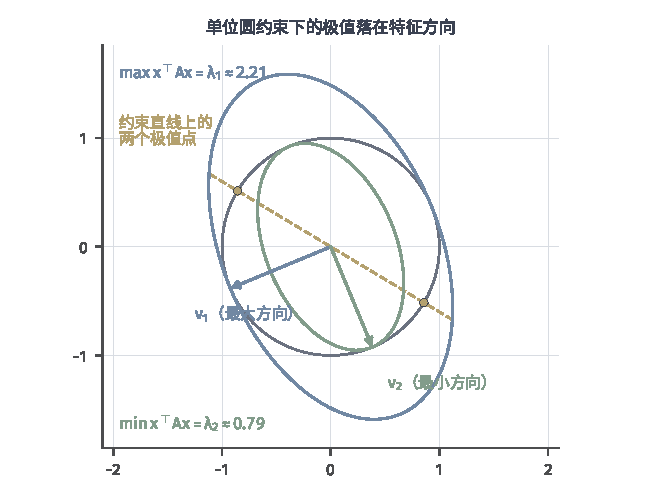
\includegraphics[width=112mm]{figures/01-mathematical-preliminaries-upper/02-linear-spaces/matplotlib/ls-sphere-constrained-extremum/ls-sphere-constrained-extremum.pdf}
  \caption{单位圆约束下的极值落在特征方向。$\bm S=\left[\begin{smallmatrix}2&0.5\\0.5&1\end{smallmatrix}\right]$，
  灰圆为$\lVert\bm x\rVert=1$。蓝椭圆$\bm x^\top\bm S\bm x=\lambda_1\approx2.21$在
  $\pm\bm v_1$处与单位圆相切（最大值），绿椭圆$=\lambda_2\approx0.79$在$\pm\bm v_2$处
  相切（最小值）；黄色虚线为子空间约束直线，其上黄点是该约束下的两个极值。
  $\lambda_{1,2}=(3\pm\sqrt2)/2$。固定复算。}
  \label{fig:ls-sphere-constrained-extremum}
\end{figure}

加权平均介于被平均各数的最小值与最大值之间，由此立即得到两端特征值的极值刻画。
\begin{theorem}[Rayleigh--Ritz]
\label{thm:matrix-analysis-rayleigh-ritz}
\label{eq:matrix-analysis-rayleigh-ritz}
设$\bm S$的特征值为$\lambda_1\geq\cdots\geq\lambda_d$，对应标准正交特征向量$\bm q_1,\ldots,\bm q_d$，则
\begin{equation*}
 \max_{\bm x\neq\bm0}R_{\bm S}(\bm x)=\lambda_1,\qquad
 \min_{\bm x\neq\bm0}R_{\bm S}(\bm x)=\lambda_d,
\end{equation*}
分别在$\bm q_1$与$\bm q_d$取到。
\end{theorem}
\begin{proof}
权重$c_i^2$非负且总和为$1$，所以$\lambda_d\leq\sum_i\lambda_ic_i^2\leq\lambda_1$；取$\bm x=\bm q_1$时只有$c_1=1$，得$\lambda_1$，取$\bm x=\bm q_d$时得$\lambda_d$。
\end{proof}
极值本身唯一，取到极值的方向却未必唯一：$\lambda_1$重复时，其特征空间中每个单位向量都给出最大值；只有在目标特征值单重时，最优方向才唯一（差一个符号）。

\paragraph{齐次最小二乘}
\label{sec:linear-algebra-homogeneous-estimation}

Rayleigh--Ritz定理的一个直接应用是带尺度约束的拟合。有时模型写成$\bm A\bm h\approx\bm0$，只关心$\bm h$各分量之间的比例。这时直接最小化$\lVert\bm A\bm h\rVert_2^2$总会得到平凡解$\bm h=\bm0$，必须先固定尺度。固定$\lVert\bm h\rVert_2=1$后得到的问题称为\term{齐次最小二乘}（homogeneous least squares）：
\begin{equation}
 \min_{\lVert\bm h\rVert_2=1}\ \lVert\bm A\bm h\rVert_2^2
 =\min_{\lVert\bm h\rVert_2=1}\bm h^\top\bm A^\top\bm A\bm h.
 \label{eq:linear-algebra-homogeneous-least-squares}
\end{equation}
右端是对称矩阵$\bm A^\top\bm A$的二次型在单位球面上的最小值。由Rayleigh--Ritz定理，最小值是$\bm A^\top\bm A$的最小特征值，最优$\bm h$是对应的单位特征向量。若$\bm A$有非零零空间，最小值为零，任一单位零空间向量都是最优解。下面的例子属于这种情形。
\begin{example}[一个方程的齐次最小二乘]
\label{ex:ls-homogeneous-least-squares-one-row}
给定一行矩阵$\bm A=[\,1\ -2\,]$。

按式~\eqref{eq:linear-algebra-homogeneous-least-squares}，最优解是$\bm A^\top\bm A$最小特征值的单位特征向量。计算得
\[
 \begin{aligned}
 \bm A^\top\bm A&=\begin{bmatrix}1&-2\\-2&4\end{bmatrix},\\
 \bm A^\top\bm A\,(2,1)^\top&=\bm0,\qquad
 \bm A^\top\bm A\,(1,-2)^\top=5\,(1,-2)^\top .
 \end{aligned}
\]
所以$\bm A^\top\bm A$的特征值为$0$与$5$。

最小特征值$0$对应的单位特征向量为$\bm h=\pm(2,1)^\top/\sqrt5$，它满足$\bm A\bm h=h_1-2h_2=0$。

结论：最小值为$0$，最优解为$\bm h=\pm(2,1)^\top/\sqrt5$；两个符号给出同一个比例$h_1:h_2=2:1$。
\end{example}

\paragraph{Courant--Fischer最小最大原理}

Rayleigh--Ritz定理只刻画两端的特征值。中间的$\lambda_k$不再是整个空间上的极值，但可以借助子空间刻画：在$k$维子空间上取Rayleigh商的最小值，再让子空间变动，取这些最小值中的最大者。

\begin{theorem}[Courant--Fischer]
\label{thm:matrix-analysis-courant-fischer}
\label{eq:matrix-analysis-courant-fischer}
对$k=1,\ldots,d$，
\begin{equation*}
 \lambda_k=\max_{\dim\mathcal V=k}\ \min_{\bm x\in\mathcal V,\bm x\neq\bm0}R_{\bm S}(\bm x)
 =\min_{\dim\mathcal W=d-k+1}\ \max_{\bm x\in\mathcal W,\bm x\neq\bm0}R_{\bm S}(\bm x).
\end{equation*}
\end{theorem}
\begin{proof}
先证第一式。取$\mathcal V_k=\operatorname{span}\{\bm q_1,\dots,\bm q_k\}$，其中单位向量的Rayleigh商是$\lambda_1,\ldots,\lambda_k$的加权平均，不小于$\lambda_k$，所以左端的最大值至少为$\lambda_k$。反过来，任取$k$维子空间$\mathcal V$，令$\mathcal W_k=\operatorname{span}\{\bm q_k,\dots,\bm q_d\}$，它是$d-k+1$维的。由维数公式，
\[
 \dim(\mathcal V\cap\mathcal W_k)\geq\dim\mathcal V+\dim\mathcal W_k-d=1,
\]
所以$\mathcal V$中有非零向量$\bm x$落在$\mathcal W_k$里。它的Rayleigh商是$\lambda_k,\ldots,\lambda_d$的加权平均，不大于$\lambda_k$，因此$\mathcal V$上Rayleigh商的最小值不超过$\lambda_k$。两方面合起来即得第一式。

第二式交换两组特征向量的角色：$\mathcal W_k$上Rayleigh商的最大值恰为$\lambda_k$；任意$d-k+1$维子空间都与$\mathcal V_k$有非零公共向量，其Rayleigh商不小于$\lambda_k$。
\end{proof}
定理只涉及子空间与Rayleigh商，不要求先知道特征向量；第~\ref{sec:ls-spectral-value-sensitivity}节正是用它比较扰动前后的特征值。同样的加权平均论证还可以一次处理$k$个方向，得到前$k$个与后$k$个特征值之和的极值刻画。

\begin{theorem}[迹极值]
\label{thm:matrix-analysis-trace-minimum}
对列标准正交的$\bm V\in\mathbb R^{d\times k}$，
\begin{equation}
 \sum_{i=d-k+1}^{d}\lambda_i\leq\operatorname{tr}(\bm V^\top\bm S\bm V)\leq\sum_{i=1}^{k}\lambda_i,
 \label{eq:matrix-analysis-trace-minimum}
\end{equation}
上下界分别由前$k$个与后$k$个特征向量张成的子空间取到。
\end{theorem}
\begin{proof}
代入$\bm S=\sum_i\lambda_i\bm q_i\bm q_i^\top$，得$\operatorname{tr}(\bm V^\top\bm S\bm V)=\sum_i\lambda_iw_i$，其中$w_i=\lVert\bm V^\top\bm q_i\rVert_2^2$。由$\bm V^\top\bm V=\bm I$得$\lVert\bm V^\top\rVert_2=1$，所以$0\leq w_i\leq1$；又$\sum_iw_i=\lVert\bm V^\top\bm Q\rVert_{\mathrm F}^2=\lVert\bm V\rVert_{\mathrm F}^2=k$。在这两个约束下，
\[
 \begin{aligned}
 \sum_i\lambda_iw_i-\sum_{i\leq k}\lambda_i
 &=\sum_{i\leq k}\lambda_i(w_i-1)+\sum_{i>k}\lambda_iw_i\\
 &\leq\lambda_k\sum_{i\leq k}(w_i-1)+\lambda_k\sum_{i>k}w_i
 =\lambda_k\Bigl(\sum_iw_i-k\Bigr)=0,
 \end{aligned}
\]
其中不等号用到$w_i-1\leq0$、$\lambda_i\geq\lambda_k$（$i\leq k$）与$w_i\geq0$、$\lambda_i\leq\lambda_k$（$i>k$）。这就是上界；对$-\bm S$应用上界即得下界。$\bm V$取前$k$个或后$k$个特征向量时，等号成立。
\end{proof}
上界说明，用$k$维子空间保留二次型的“能量”，最好的选择是前$k$个特征方向，这是主成分分析的代数基础。

\paragraph{广义特征问题}

有时长度不按欧氏范数度量，而按第~\ref{sec:ls-weighted-inner-products}节的加权内积度量，约束$\lVert\bm x\rVert_2=1$相应地换成$\bm x^\top\bm B\bm x=1$（$\bm B\succ0$），要比较的是广义Rayleigh商$\bm x^\top\bm S\bm x/\bm x^\top\bm B\bm x$。它可以化回普通情形。由定理~\ref{thm:ls-gram-factor}写$\bm B=\bm L^\top\bm L$，$\bm L$可逆，令$\bm z=\bm L\bm x$，则$\bm x^\top\bm B\bm x=\bm z^\top\bm z$，而
\[
 \frac{\bm x^\top\bm S\bm x}{\bm x^\top\bm B\bm x}
 =\frac{\bm z^\top\bm L^{-\top}\bm S\bm L^{-1}\bm z}{\bm z^\top\bm z}
\]
是对称矩阵$\bm L^{-\top}\bm S\bm L^{-1}$的普通Rayleigh商。其特征方程$\bm L^{-\top}\bm S\bm L^{-1}\bm z=\mu\bm z$左乘$\bm L^\top$并换回$\bm v=\bm L^{-1}\bm z$，就是下面的方程。
\begin{definition}[广义特征值]
\label{def:matrix-analysis-generalized-eigenvalue}
对实对称$\bm S$与$\bm B\succ0$，称满足
\begin{equation}
 \bm S\bm v=\mu\bm B\bm v,\qquad\bm v\neq\bm0
 \label{eq:matrix-analysis-generalized-eigenproblem}
\end{equation}
的$\mu$为广义特征值，$\bm v$为广义特征向量，求解它们的问题称为\term{广义特征问题}（generalized eigenvalue problem）。
\end{definition}
对$\bm L^{-\top}\bm S\bm L^{-1}$应用谱定理可知：广义特征值全为实数；广义特征向量可以取为$\bm B$正交的，即$\bm v_i^\top\bm B\bm v_j=\delta_{i,j}$（因为$\bm z_i=\bm L\bm v_i$标准正交）；最大、最小广义特征值就是广义Rayleigh商的最大、最小值。

计算时也应走这条换元的路。直接对$\bm B^{-1}\bm S$求特征值虽然得到同样的$\mu$，但$\bm B^{-1}\bm S$一般不对称，会丢掉对称结构带来的正交性与数值稳定性。

\subsection{对称矩阵的函数}
\label{sec:ls-matrix-functions}
\label{sec:matrix-analysis-functions-structured-operations}

多项式$p(\bm S)$可以直接用矩阵的幂与加法算出。平方根、对数、指数这类非多项式函数怎样作用于矩阵？谱定理提示了做法。由$\bm S=\bm Q\bm\Lambda\bm Q^\top$与$\bm Q^\top\bm Q=\bm I$，连乘时相邻的$\bm Q^\top\bm Q$相消，得$\bm S^k=\bm Q\bm\Lambda^k\bm Q^\top$；再按系数相加，得$p(\bm S)=\bm Q\,p(\bm\Lambda)\,\bm Q^\top$。也就是说，多项式在每个特征方向上只作用于对应的特征值。把这一观察作为定义，推广到一般函数。

\paragraph{沿特征方向的定义}

设$\bm S=\bm Q\bm\Lambda\bm Q^\top$，$f$是定义在全部特征值$\lambda_i$上的实函数，令
\begin{equation}
 f(\bm S)=\bm Q\operatorname{diag}\bigl(f(\lambda_1),\ldots,f(\lambda_d)\bigr)\bm Q^\top.
 \label{eq:ls-symmetric-spectral-function}
\end{equation}
$\bm Q$不唯一，需要检查结果是否依赖它的选取。把同一特征值$\lambda$的特征向量归为一组，$\sum_{\lambda_i=\lambda}\bm q_i\bm q_i^\top$是到特征空间$\ker(\bm S-\lambda\bm I)$的正交投影$\bm P_\lambda$，它只依赖这个子空间，与子空间内基的选取无关。于是$f(\bm S)=\sum_\lambda f(\lambda)\bm P_\lambda$，求和遍历不同的特征值，结果由$\bm S$唯一确定。$f(z)=z^k$时，定义回到矩阵幂$\bm S^k$，与已有运算相容。

矩阵函数作用在特征方向上，而不是逐元素作用。下面的例子对照这两种做法。
\begin{example}[矩阵平方根与逐元素开方]
\label{ex:ls-matrix-square-root-two-by-two}
给定示例~\ref{ex:ls-symmetric-spectral-two-by-two}的$\bm S=3\bm q_1\bm q_1^\top+\bm q_2\bm q_2^\top$，取$f(z)=\sqrt z$。按式~\eqref{eq:ls-symmetric-spectral-function}，
\[
 f(\bm S)=\sqrt3\,\bm q_1\bm q_1^\top+\bm q_2\bm q_2^\top
 =\frac12\begin{bmatrix}\sqrt3+1&\sqrt3-1\\\sqrt3-1&\sqrt3+1\end{bmatrix}.
\]
它的平方为
\[
 \frac14\begin{bmatrix}(\sqrt3+1)^2+(\sqrt3-1)^2&2(\sqrt3+1)(\sqrt3-1)\\2(\sqrt3+1)(\sqrt3-1)&(\sqrt3+1)^2+(\sqrt3-1)^2\end{bmatrix}
 =\frac14\begin{bmatrix}8&4\\4&8\end{bmatrix}=\bm S .
\]
逐元素开方得到$\left[\begin{smallmatrix}\sqrt2&1\\1&\sqrt2\end{smallmatrix}\right]$，它的平方是$\left[\begin{smallmatrix}3&2\sqrt2\\2\sqrt2&3\end{smallmatrix}\right]\neq\bm S$。结论：沿特征方向定义的$f(\bm S)$满足$f(\bm S)^2=\bm S$，逐元素开方的结果则不满足。
\end{example}

\paragraph{平方根、实幂与对数}

$\bm S$半正定时，全部$\lambda_i\geq0$，可取$f(z)=\sqrt z$，得到\term{矩阵平方根}（matrix square root）
\[
 \bm S^{1/2}=\bm Q\operatorname{diag}(\sqrt{\lambda_1},\ldots,\sqrt{\lambda_d})\bm Q^\top ,
\]
它半正定且$(\bm S^{1/2})^2=\bm S$。

方程$\bm X^2=\bm S$一般有多个解，例如$\bm I$与$-\bm I$的平方都是$\bm I$；但要求$\bm X$半正定后，解是唯一的。设半正定的$\bm X=\sum_j\mu_j\bm p_j\bm p_j^\top$（$\mu_j\geq0$，$\bm p_j$标准正交）满足$\bm X^2=\bm S$，则$\bm S=\sum_j\mu_j^2\bm p_j\bm p_j^\top$，即每个$\bm p_j$都是$\bm S$的特征向量，特征值为$\mu_j^2$。于是$\bm S$的$\lambda$特征空间恰由满足$\mu_j^2=\lambda$的那些$\bm p_j$张成，而$\mu_j\geq0$迫使这些$\mu_j=\sqrt\lambda$。所以$\bm X$在$\bm S$的每个特征空间上都乘以$\sqrt\lambda$，这正是$\bm S^{1/2}$的作用，$\bm X=\bm S^{1/2}$。

$\bm S$正定时，全部$\lambda_i>0$，还可以取任意实幂$\bm S^\alpha$，例如$\alpha=-1/2$给出逆平方根；也可以取\term{矩阵对数}（matrix logarithm）$\log\bm S=\bm Q\operatorname{diag}(\log\lambda_1,\ldots,\log\lambda_d)\bm Q^\top$。有零特征值时，负幂与对数都没有定义。注意$\log\bm S$是矩阵，而$\log\det\bm S=\sum_i\log\lambda_i=\operatorname{tr}(\log\bm S)$是标量，二者不能混淆。

按定义计算需要完整的谱分解，代价较高。若只需计算$\lVert\bm S^{1/2}\bm x\rVert_2$或作用$\bm S^{-1/2}$做白化，可以用定理~\ref{thm:ls-gram-factor}的因子代替平方根：写$\bm S=\bm L^\top\bm L$，则$\lVert\bm L\bm x\rVert_2^2=\bm x^\top\bm S\bm x=\lVert\bm S^{1/2}\bm x\rVert_2^2$，两者给出同样的长度。第~\ref{chap:linear-equations-and-optimization}章的Cholesky分解把$\bm L$取成三角矩阵，那时作用$\bm L^{-1}$只需解三角方程。

至此，本节的问题有了回答。能用正交矩阵对角化的实矩阵，即具有一组标准正交特征向量的实矩阵，恰好是对称矩阵；谱分解$\bm S=\bm Q\bm\Lambda\bm Q^\top$把它写成沿互相垂直方向的伸缩。特征值同时是Rayleigh商的极值与最小最大值，可以只凭二次型来比较；矩阵函数沿特征方向逐个作用于特征值。但许多重要的方阵并不对称，例如平面旋转与示例~\ref{ex:ls-triangular-power}的上三角矩阵$\left[\begin{smallmatrix}0.8&4\\0&0.5\end{smallmatrix}\right]$。下一节讨论，对一般方阵，坚持用正交矩阵换基时最多能化到多简单。
